\documentclass[11pt]{report}
%
%
%--------------------   start of the 'preamble'
%
\usepackage{graphicx,amssymb,amstext,amsmath}
\usepackage[spanish,activeacute]{babel}
\usepackage{graphicx}
\usepackage{epsfig}
\usepackage{subfigure}
\usepackage{url}
\usepackage[colorlinks=true]{hyperref}

%---------------------   end of the 'preamble'
%
\begin{document}
%-----------------------------------------------------------
\title{\textbf{\huge{Taller: Introducci'on a R}}}
\author{Blanca A. Vargas Govea\\\texttt{blanca.vg@gmail.com}}
\date{}
\maketitle
%-----------------------------------------------------------
% \begin{abstract}\centering
% Taller de introducci'on a R.
% \end{abstract}
%-----------------------------------------------------------
\tableofcontents
%-----------------------------------------------------------
\chapter{Introducci'on}

%-----------------------------------------------------------
\section{Instalaci'on}
\begin{itemize}
    \item Instalar R~\cite{Rproject} . Disponible para Linux, MacOS X y Windows:\\
 en \url{http://cran.r-project.org/mirrors.html}.
    \item Puede usarse en consola o instalar un IDE.\\
Sugerencia: RStudio \url{http://www.rstudio.org/}.
\end{itemize}

El conjunto de datos que se usar'a es credit-g.csv~\cite{credit:2010}.

En modo consola:
\begin{verbatim}
$ R
\end{verbatim}

%-----------------------------------------------------------
\section{C'omo obtener ayuda}
\begin{verbatim}
help.start()        # ayuda general
help(nombrefuncion) # detalles sobre la funcion
?funcion            # igual que el anterior
apropos("solve")    # lista las funciones que contienen "solve"
example(solve)      # muestra un ejemplo del uso de solve
help("*")
vignette()           
vignette("foo")     
data()              # muestra los conjuntos de datos disponibles
help(datasetname)   # detalles del conjunto de datos
\end{verbatim}

%-----------------------------------------------------------
\section{Espacio de trabajo}
Es el entorno de tu sesi'on actual en R e incluye cualquier objeto: vectores, matrices, dataframes, listas, funciones. Al finalizar la sesi'on se puede guardar el actual espacio de trabajo para que autom'aticamente se cargue en la siguiente.

Algunos comandos est'andar para definir el espacio de trabajo son los siguientes:

\begin{verbatim}
getwd() # muestra el directorio actual
ls()    # lista los objetos en el espacio de trabajo
setwd(mydirectory)      # cambia el path a mydirectory
setwd("c:/docs/mydir")  # notar / en vez de \ en Windows
setwd("/usr/rob/mydir") # en Linuz
history() # despliega los 25 comandos recientes
history(max.show=Inf) # despliega los comandos previos
q() # quit R. 
\end{verbatim}

\section{Packages}
\begin{verbatim}
.libPaths() # obtiene ubicación de la librería
library()   # muestra los paquetes instalados
search()    # muestra los paquetes cargados
# descarga e instala paquetes del repositorio CRAN
install.packages("nombredelpaquete")  
library(package) # carga el paquete
\end{verbatim}

\section{Scripts}
\begin{verbatim}
# en Linux
R CMD BATCH [options] my_script.R [outfile] 

# en ms windows (ajustar el path a R.exe)
"C:\Program Files\R\R-2.5.0\bin\R.exe" CMD BATCH
   --vanilla --slave "c:\my projects\my_script.R" 

source("myfile")
sink("record.lis") # direcciona la salida al archivo record.lis
\end{verbatim}

%http://cran.r-project.org/doc/manuals/R-intro.html#Data-permanency-and-removing-objects
%http://www.statmethods.net/input/index.html
%http://www.cyclismo.org/tutorial/R/input.html
%-----------------------------------------------------------



\chapter{Tipos de datos y funciones b'asicas}

%-----------------------------------------------------------
\section{N'umeros}

\begin{verbatim}
var1 <- 54
var1

var2 <- sqrt(var1*8)
var2
\end{verbatim}
%-----------------------------------------------------------
\section{Vectores}

\begin{verbatim}
vector <- c(1,2,3,4,5)
vector[0]
vector[1]

cadena <- "uno"
cadena

lcadena <- c("casa","manzana","uva")
lcadena

vlogico <- c(TRUE,FALSE,TRUE,TRUE,FALSE)
vlogico
\end{verbatim}

%-----------------------------------------------------------
\section{Dataframes}

\begin{verbatim}
c1 <- c(25,26,27,28)
c2 <- c("Ana", "Lola", "Luis", "Pedro")
c3 <- c(TRUE,TRUE,TRUE,FALSE)
mydata <- data.frame(c1,c2,c3)
names(mydata) <- c("ID","Nombre","Aprobado") # nombres de variables
\end{verbatim}

Otros tipos de datos son: arrays, listas y factores.
%-----------------------------------------------------------
\section{Exportar e importar datos}
\begin{verbatim}
    > setwd("path_name")
    > credit <- read.csv(file = "../data/credit-g.csv", sep = ",",
                         na.strings = "NULL")
\end{verbatim}
%-----------------------------------------------------------
\section{Despliegue de objetos}
\begin{verbatim}
ls()  # lista de objetos
names(credit) # variables de credit
str(credit) # estructura de credit
levels(credit$foreign_worker) # niveles(valores de variable)
dim(credit) # dimensiones (ren x cols)
class(credit) # clase del objeto
credit  # objeto
head(credit, n=10)
tail(credit, n=10)
credit$purpose
#purpose
attach(credit)  # coloca la bd en el path
purpose
\end{verbatim}
%-----------------------------------------------------------
\section{Renglones, columnas, m'inimo y m'aximo}

\begin{verbatim}
# Explorando conteo
ren <- nrow(credit)   # raw row count
col <- ncol(credit)

# Min y Max 
agemin <- min(age,na.rm = TRUE) # min sin NULLS en age
agemax <- max(age,na.rm = TRUE)

ammin <- min(credit_amount,na.rm = TRUE) # min sin NULLS en age
ammax <- max(credit_amount,na.rm = TRUE)
\end{verbatim}
%-----------------------------------------------------------
\section{Subconjuntos}

\begin{verbatim}
# Filtrando por edad
mayor30 <- subset(credit, age >= 30)
renmayor30 <- nrow(mayor30)
renmayor30

en20y40 <- subset(credit, age >= 20  & age <= 40)
ren20y40 <- nrow(en20y40)
ren20y40
\end{verbatim}

%-----------------------------------------------------------
\subsection{Muestra aleatoria}

\begin{verbatim}
set.seed(32) 
dsmall <- credit[sample(nrow(credit), 10), ]
dsmall
\end{verbatim}

%-----------------------------------------------------------
\subsection{Definiendo rangos}
\begin{verbatim}
# Filtrando por bins 
agebin = cut(age,breaks = c(18,30,40,50,60,70,80))
agebinfile <- data.frame(purpose,credit_amount,personal_status,
              housing,job,age=agebin,class)
agebinfile
\end{verbatim}

%-----------------------------------------------------------
\section{'Unicos, frecuencia, orden}
\begin{verbatim}
# unicos
unicos <- unique(class)
unicos
nhousing <- length(unique(class))
nhousing
\end{verbatim}

\begin{verbatim}
# table
mycredit <- table(dsmall$class)
mycredit
mycredit <- table(dsmall$age,dsmall$credit_amount)
mycredit
\end{verbatim}

\begin{verbatim}
# ordenar
mycredit <- table(dsmall$housing)
mycredit
mylist <- sort(mycredit,decreasing = TRUE)
mylist
\end{verbatim}

%-----------------------------------------------------------
\section{Construyendo archivos de salida}

\begin{verbatim}
oframe = data.frame(purpose,credit_amount,personal_status,
                    housing,job,age=agebin,class)
write.table(oframe, row.names = FALSE, 
            sep = ";",quote = FALSE, file="../data/output01_data.csv")
\end{verbatim}

\chapter{An'alisis descriptivo}

%-----------------------------------------------------------
\section{Conceptos b'asicos}
%%%%%%%%%%%%%%%%%%%%%%%%%%%%%%%%%%%%%%%%%%%%%%%%%%%%%%%%
%descan1.pdf pr'actico totalmente%

%GUIAS PRACTICAS%
%Chapter 4 Descriptive statistics and R graphics. Usar como gu'ia.%
%http://www.r-bloggers.com/r-tutorial-series-summary-and-descriptive-statistics/
%http://geography.uoregon.edu/bartlein/old_courses/geog414f03/lectures/lec04.htm
%http://www.dissertation-statistics.com/population-sample.html
%http://www.socialresearchmethods.net/kb/sampstat.htm

El an'alisis descriptivo o exploratorio tiene por objetivo describir los datos mediante t'ecnicas estad'isticas y gr'aficas. El an'alisis descriptivo nos da un primer acercamiento a los datos y extrae caracter'isticas importantes que se utilizar'an para an'alisis posteriores. Este tipo de an'alisis es una herramienta 'util para encontrar errores, ver patrones en los datos, encontrar y generar hip'otesis. A continuaci'on se describen conceptos b'asicos~\cite{st1,st2,st3,staplicaciones} que se utilizan a lo largo del documento.


\begin{description}
%-----------------------
\item [Poblaci'on] \hfill \\
Es el conjunto completo de elementos de nuestro inter'es. Las caracter'isticas de una poblaci'on son las medidas estad'isticas de cada uno de sus elementos.

\item [Muestra] \hfill \\
Es una proporci'on de la poblaci'on. Una muestra posee las mismas caracter'isticas de la poblaci'on si se obtiene aleatoriamente. Las muestras aleatorias deben cumplir con dos caracter'isticas: 1) todos los elementos deben tener la misma oportunidad de ser seleccionados y 2) la selecci'on de un elemento debe ser independiente de la selecci'on de otro. 

La diferencia entre una poblaci'on y una muestra es que con la poblaci'on, nuestro inter'es es identificar sus caracter'isticas mientras que con la muestra, nuestro inter'es es hacer inferencias sobre las caracter'isticas de la poblaci'on. Si la medida (e.g, media, mediana) se obtiene de la poblaci'on completa, se le llama \textbf{par'ametro} mientras que si se obtiene de una muestra, se le llama \textbf{estimaci'on}.

\item [Estad'istica descriptiva] \hfill \\
Describe los datos sin ning'un tipo de generalizaci'on. Ejemplo: porcentaje de menores de edad que utilizan redes sociales.

\item [Inferencia estad'istica] \hfill \\
Generaliza o induce algunas propiedades de la poblaci'on a partir de la cual los datos se tomaron. Ejemplo: \textquestiondown es la satisfacci'on del usuario de sistemas de recomendaci'on significativamente diferente entre hombres y mujeres?

\item [Variables categ'oricas] \hfill \\
No aparecen de forma num'erica y tienen dos o m'as categor'ias o valores. Pueden ser nominales y ordinales. Una variable nominal no tiene un orden (e.g., rojo, amarillo, suave), mientras que la ordinal designa un orden (e.g., primer lugar, segundo lugar).

\item [Variables num'ericas] \hfill \\
Son aquellas que pueden tomar cualquier valor dentro de un intervalo finito o infinito. Hay dos tipos de variable num'erica: de intervalo y radio. Una variable de intervalo tienen valores cuyas diferencias son interpretables pero no tienen un cero verdadero, un ejemplo es la temperatura. Pueden ser sumadas o restadas pero no multiplicadas o divididas (e.g., hoy no es el doble de c'alido que ayer). Una variable de radio tiene un cero verdadero y pueden sumarse, multiplicarse o dividirse (e.g., el peso).

Para cada tipo de variable hay diferentes t'ecnicas de an'alisis.
\end{description}

El an'alisis puede ser \textbf{univariable}, en el cual se exploran las variables o atributos uno por uno o \textbf{bivariable}, en el cual simult'aneamente se analizan dos variables para conocer la relaci'on entre ellas, su fuerza o si hay diferencias entre 'ellas y el significado de las mismas. El an'alisis bivariable puede ser entre dos variables num'ericas, dos variables categ'oricas y una vari'able num'erica y una categ'orica.
Los valores estad'isticos de las variables son las caracter'isticas  que se extraer'an de los perfiles de usuario e 'items.

\section{An'alisis univariable}
En este tipo de an'alisis se exploran las variables una por una y dependiendo de su tipo (i.e., categ'orica, num'erica) se aplican distintos tipos de an'alisis y gr'aficas.

Para las \textbf{variables categ'oricas} el an'alisis exploratorio b'asicamente es un conteo del n'umero de valores de la variable especificada y el porcentaje de valores de la variable espec'ifica. Se utilizan las gr'aficas de barras y de pay. Por otro lado, las \textbf{variables num'ericas} se analizan calculando el m'inimo, m'aximo, media, mediana, moda, rango, los cuantiles, la varianza, la desviaci'on est'andar, el coeficiente de variaci'on, la asimetr'ia y la curtosis. Se visualizan mediante histogramas y gr'aficas de caja.

%Diferencia entre histogramas y gr'aficas de barra: las gr'aficas de barra se usan para mostrar la frecuencia o proporci'on de las variables categ'oricas. Traducen los datos de tablas de frecuencia a una representaci'on visual. Un histograma se usa para visualizar la distribuci'on de las variables cont'inuas y el tama\~{n}o del bin es importante.

El conjunto de medidas son las caracter'isticas que nos interesan para el modelo que queremos obtener por lo que es importante recordar lo que cada una representa. 

%http://www.chem.utoronto.ca/coursenotes/analsci/StatsTutorial/MeasMeanVar.html
\begin{description}
%-----------------------
\item [Media] \hfill \\
La media, en estad'istica, puede tener dos significados: la media aritm'e-\linebreak es una medida de tendencia central de un espacio muestral. En un conjunto de datos, es la suma de una lista dividida por el n'umero de miembros de la lista. Se denota por $\bar{x}$ o $\mu$ y puede verse como la salida esperada $E(x)$ de un evento $x$ tal que si la medida se realiza varias veces, el valor promedio ser'ia la salida m'as com'un.

\[
    \bar{x} =\frac{1}{n}\sum_{i=1}^{n}x_i = \frac{1}{n}(x_1+x_2+...+x_n)
\]

La media describe la ubicaci'on central de los datos y la desviaci'on est'andar describe la dispersi'on. La media de una muestra puede ser diferente de la media poblacional especialmente para muestras peque\~{n}as pero a mayor tama~{n}o de la muestra, es m'as probable que la media muestral se acerque a la media poblacional.

Es el primer momento de la distribuci'on de una variable aleatoria. Un momento es una medida cuantitativa de la forma de un conjunto de puntos.

No es una medida muy robusta para describir la tendencia central de un conjunto de datos pues es f'acilmente influenciada por valores at'ipicos. Para distribuciones asim'etricas la media no concuerda con el centro por lo que en esos casos se prefiere la media para describir la tendencia central.

%-----------------------
\item [Mediana] \hfill \\
Es el n'umero que separa el conjunto de datos por la mitad. Para encontrarla se ordenan los n'umeros en orden ascendente o descendente y se escoge el que est'a a la mitad. Si la lista tiene un n'umero par de elementos, la mediana se calcula obteniendo la media de los n'umeros centrales. Para cualquier distribuci'on de probabilidad , la mediana satisface las siguientes desigualdades:

\begin{center}
$    Pr(X \leq m) \geq \frac{1}{2} $
y 
$
    Pr(X \geq m) \geq \frac{1}{2}
$
\end{center}

Puede usarse como medida de localizaci'on de tendencia central cuando una distribuci'on es asim'etrica. Es igual al segundo cuartil.
%-----------------------
\item [Moda] \hfill \\
La moda es el valor que ocurre con mayor frecuencia en un conjunto de datos. Puede diferir mucho de la media y mediana debido a la asimetr'ia de las distribuciones.
%-----------------------
\item [Rango] \hfill \\
El rango es la diferencia entre los valores m'aximo y m'inimo de valores en un conjunto. Como solamente depende de dos observaciones es una medida d'ebil de la dispersi'on excepto si la muestra es grande.
%-----------------------
%http://stattrek.com/AP-Statistics-1/Boxplot.aspx
%http://www.estadisticaparatodos.es/taller/graficas/cajas.html

\item [Varianza y desviaci'on est'andar] \hfill \\
La varianza describe que tan lejos est'an los valores de la media. La varianza y la desviaci'on est'andar ($\sigma$ y $\sigma^2$ respectivamente) son indicadores de la dispersi'on de los datos dentro de una muestra o poblaci'on. Como en el caso de la media, la varianza de la poblaci'on y desviaci'on est'andar son las desviaciones esperadas. La varianza de una poblaci'on se calcula usando la media de una poblaci'on:

\[
    \sigma^2 = \frac{1}{n}\sum_{i=1}{(x_i - \mu)}^2
\]

Para calcular la varianza muestral, encontramos los errores de todas las mediciones, 'esto es, la diferencia entre cada medida y la media muestral, $x_i - \bar{x}$. Luego se eleva al cuadrado cada valor y se suman, se divide entre el n'umero de observaciones menos $1$. La desviaci'on est'andar muestral es la ra'iz cuadrada de la varianza muestral $\sqrt{s^2}$. %La varianza muestral usa un grado de libertad de $n-1$ porque se pierde un grado de libertad al estimar la media de la poblaci'on con la media muestral.

Es el segundo momento de una distribuci'on.


\item [Cuantiles] \hfill \\
Son puntos tomados en intervalos regulares de la distribuci'on acumulativa de una variable aleatoria. Dado un conjunto de datos ordenados, los cuantiles-q dividen el conjunto en q subconjuntos de igual tama\~{n}o; son los valores que marcan los l'imites entre subconjuntos consecutivos. Los casos especiales son: cuartiles, decentiles, centiles y percentiles.

\medskip
\textbf{Cuartiles}. Un cuartil es cualquiera de los tres valores que dividen los datos ordenados en cuatro partes iguales. El primer cuartil (Q1) de un grupo de valores es el valor en el que cae el $25$\% de los datos. El segundo cuartil Q2 es la mediana (el $50$\% de los datos). El tercer cuartil Q3 de un grupo de valores es en el que cae el $75$\% de los datos. La distancia entre el primero y el tercer cuartiles se conoce como el rango inter-cuartil RIC (Q3-Q1) y a veces se usa como una alternativa robusta a la desviaci'on est'andar.

Una gr'afica muy 'util para visualizar los cuartiles son los diagramas de caja; se les conoce tambi'en como diagramas de caja y bigotes (Figura~\ref{fig:bigotes}). Este tipo de gr'afica resume las siguientes medidas: mediana, cuartiles superior e inferior y valores m'inimo y m'aximo. La caja contiene el $50$\% central de los datos. La parte superior de la caja representa el $75$ percentil de los datos . La l'inea central representa la mediana y el primer y tercer cuartiles son las orillas de la caja. El 'area de la caja es el rango intercuartil. Los valores extremos, dentro de $1.5$ veces del rango intercuartil son los extremos de las l'ineas. Los puntos a mayor de $1.5$ veces el IQR de la mediana son potenciales valores at'ipicos. 

\begin{figure}[h]
    \begin{center}
    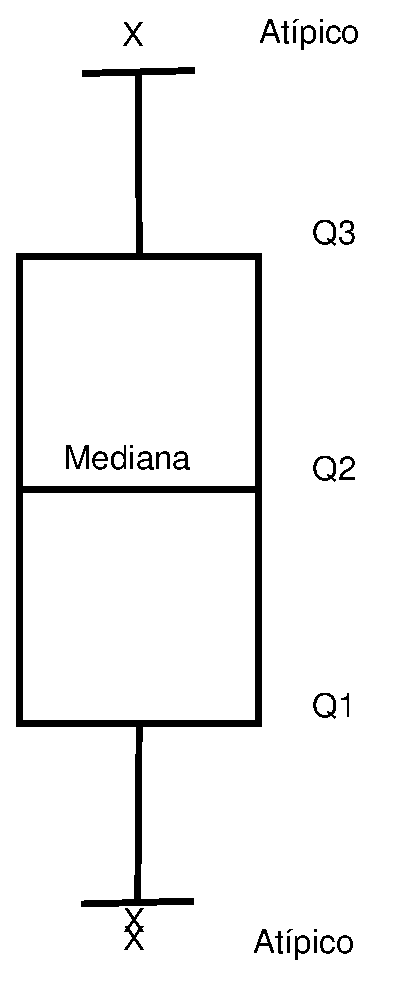
\includegraphics[height=5cm,keepaspectratio]{theimg/boxplotdia}
    \caption[Diagrama de caja y bigotes]{Diagrama de caja y bigotes}
    \label{fig:bigotes}
    \end{center}
\end{figure}

\medskip
\textbf{Valores at'ipicos}. Un valor at'ipico es una observaci'on num'ericamente distante del resto de los datos y puede representar datos err'oneos. Tomando como referencia la diferencia entre el primer cuartil (Q1) y el tercer cuartil Q3, o valor intercuartil, en un diagrama de caja se considera un valor atípico el que se encuentra 1,5 veces esa distancia de uno de esos cuartiles (at'ipico leve) o a 3 veces esa distancia (atípico extremo).

%Para ello se calcula cuándo se consideran atípicos los valores. Son aquellos inferiores a Q1-1.5*RIC o superiores a Q3+1.5*RIC.

%Además, se pueden considerar valores extremadamente atípicos aquellos que exceden Q1-3*RIC o Q3+3*RIC.

%\item [Coeficiente de variaci'on]
\item [Asimetr'ia]\hfill \\
Es una medida de la asimetr'ia de una distribuci'on que se define por la siguiente f'ormula:

\begin{center}
$\gamma_1 = \mu_3/{\mu_2}^{3/2}$
\end{center}

El valor puede ser positivo, negativo o indefinido.  Como regla, una asimetr'ia negativa indica que la media de los datos es menor que la mediana y la distribuci'on est'a concentrada a la izquierda; la asimetr'ia positiva indica que la media es mayor que la mediana y la distribuci'on est'a concentrada a la derecha. Esta regla aplica solamente a distribuciones unimodales cuyos histogramas tienen un solo pico. Cualitativamente, una asimetr'ia negativa indica que la cola del lado izquierdo de la distribuci'on de probabilidad es m'as larga que la cola derecha y el grueso de los valores, incluyendo la mediana cae en el lado derecho de la media. Una asimetr'ia positiva indica lo contrario. Un valor de cero indica que los valores son relativamente distribuidos igual a ambos lados de la media. Es el tercer momento de la media. Conocer la asimetr'ia del conjunto de datos indica si las desviaciones de la media ser'an positivas o negativas.

\item [Curtosis]\hfill \\
Es el cuarto momento central y mide si la distribuci'on es alta y delgada o corta y gruesa en comparaci'on a la distribuci'on normal de la misma varianza. Puede decirse que la curtosis mide qu'e tan puntiaguda es la distribuci'on. Valores altos de curtosis indican que la varianza es el resultado de desviaciones extremas infrecuentes. Se define como:

\begin{center}
$\gamma_2 = \frac{\mu_4}{\delta^4} - 3$ 
\end{center}

Una distribuci'on con curtosis elevada tiene un pico agudo y largo, colas anchas, mientras que con baja curtosis tieen picos m'as redondeados y colas m'as delgadas y cortas.
\end{description}

%-----------------------------------------------------------
\section{En R}
\begin{verbatim}
> setwd("path_name")
> credit <- read.csv(file = "../data/credit-g.csv", sep = ",",
                     na.strings = "NULL")
> attach(credit)
\end{verbatim}

Cargar librer'ia moments
\begin{verbatim}
install.packages("moments")
library(moments)      
\end{verbatim}

%-----
\subsection{Moda}
\begin{verbatim}
Mode <- function (x) {
    cngtable <- table(x)
    n <- length(cngtable)
    mode <- as.double(names(sort(cngtable)[n]))
    mode
}

moda <- Mode(age)
moda
\end{verbatim}
%-----
\subsection{Rango}
\begin{verbatim}
Rng <- function(x) {
    rangem <- diff(range(x))
    rangem
}

rango <- Rng(age)
rango
\end{verbatim}
%-----
\subsection{Cuantiles}
\begin{verbatim}
Quantiles <- function(x) {
    quants <- quantile(x)
    quantval <- as.double(names(table(quants)))
    quantval
}

q <- Quantiles(sort(age))
q
\end{verbatim}

%-----
\subsection{Media}
\begin{verbatim}
media <- round(mean(age),2)
media
\end{verbatim}

%-----
\subsection{Mediana}
\begin{verbatim}
mediana <- round(median(age),2)
mediana
\end{verbatim}

%-----
\subsection{Varianza}
\begin{verbatim}
varianza <- round(var(age),2)
varianza
\end{verbatim}

%-----
\subsection{Desviaci'on est'andar}

\begin{verbatim}
sd <- round(sd(age),2)
sd
\end{verbatim}

%-----
\subsection{Curtosis}
\begin{verbatim}
kurtosis <- round(kurtosis(age),2)
kurtosis
\end{verbatim}

%\begin{verbatim}
%# Skewness
%sk <- round(skewness(age),2)
%sk
%\end{verbatim}



\chapter{Gr'aficas}

%-----------------------------------------------------------
\section{Gr'aficas est'andar}

\begin{verbatim}
setwd("path")
credit <- read.csv(file = "../data/credit-g.csv", sep = ",", 
          na.strings = "NULL")
attach(credit)

set.seed(32) # Muestra
dsmall <- credit[sample(nrow(credit), 5), ]
dsmall
\end{verbatim}

%-----
\subsection{Puntos}

\begin{verbatim}
png(filename = "../figures/foo1.png") # puntos
plot(age,credit_amount)
\end{verbatim}

\begin{verbatim}
png(filename = "../figures/foo1b.png")
plot(dsmall$age,type= "o",col="blue")
\end{verbatim}

\begin{verbatim}
png(filename = "../figures/foo1c.png")
plot(dsmall$existing_credits, type="o", col="blue", ylim=c(0,12))
lines(dsmall$residence_since, type="o", pch=22, lty=2, col="red")
legend(7,12, c("existing_credits","residence_since"), 
   col=c("blue","red"), pch=21:22, lty=1:2)
\end{verbatim}

\begin{figure}[h]
 \begin{center}
 \subfigure[foo1]{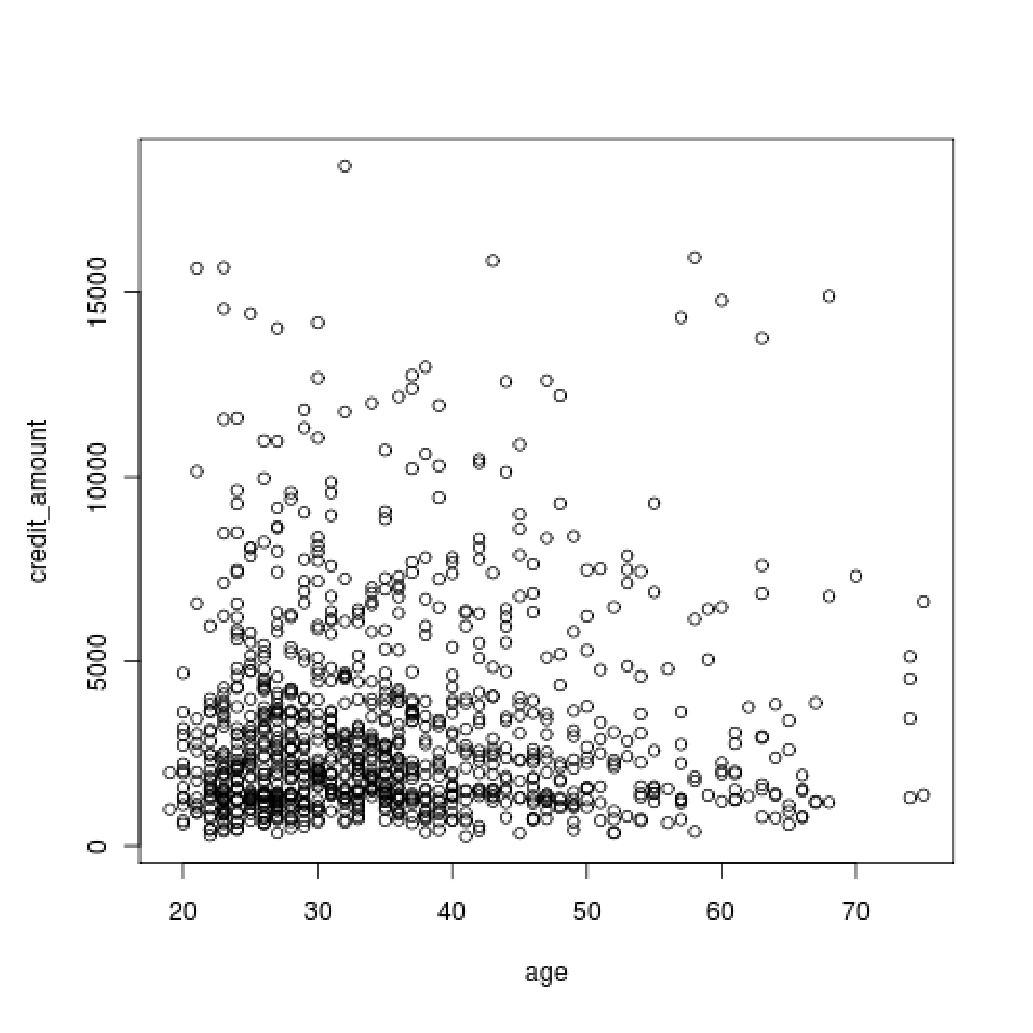
\includegraphics[keepaspectratio,width=4cm]{theimg/foo1}}
 \hspace{0.1cm}
 \subfigure[foo1b]{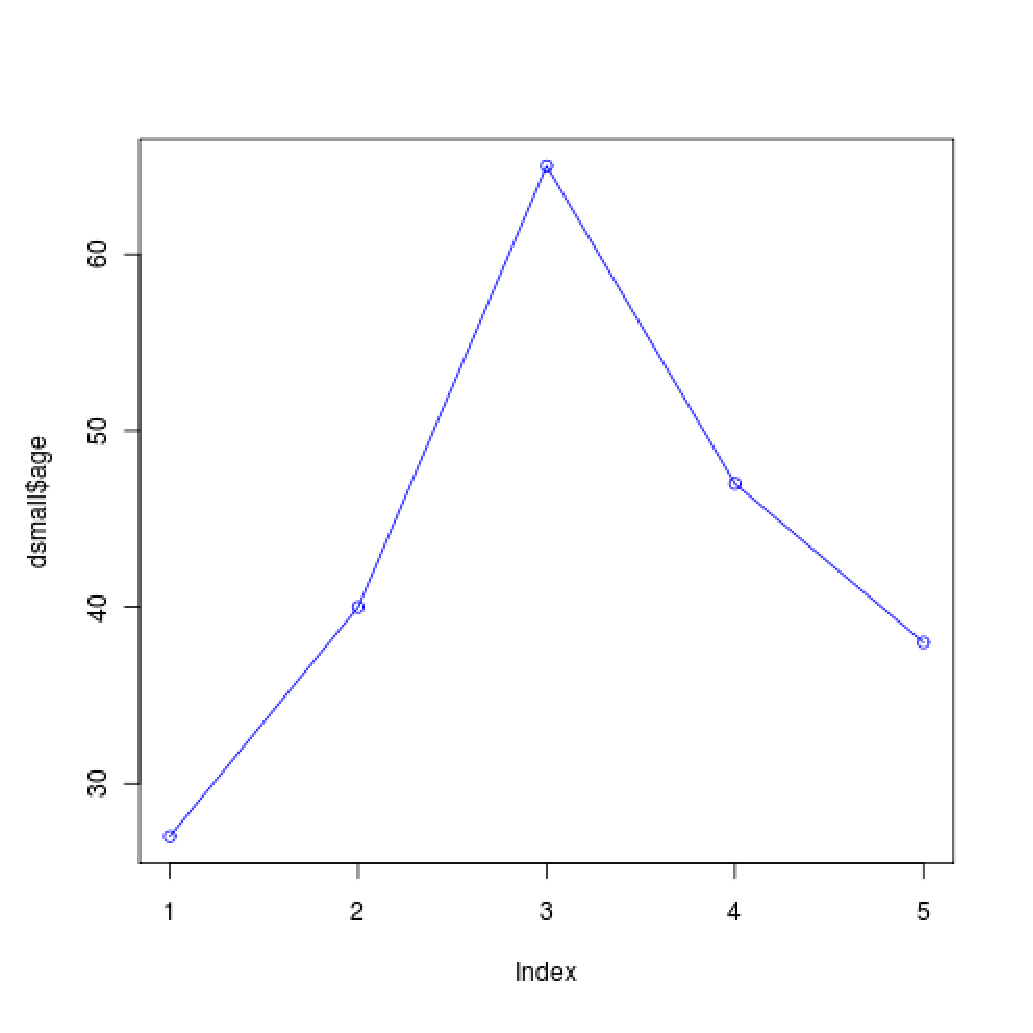
\includegraphics[keepaspectratio,width=4cm]{theimg/foo1b}}
 \hspace{0.1cm}
 \subfigure[foo1c]{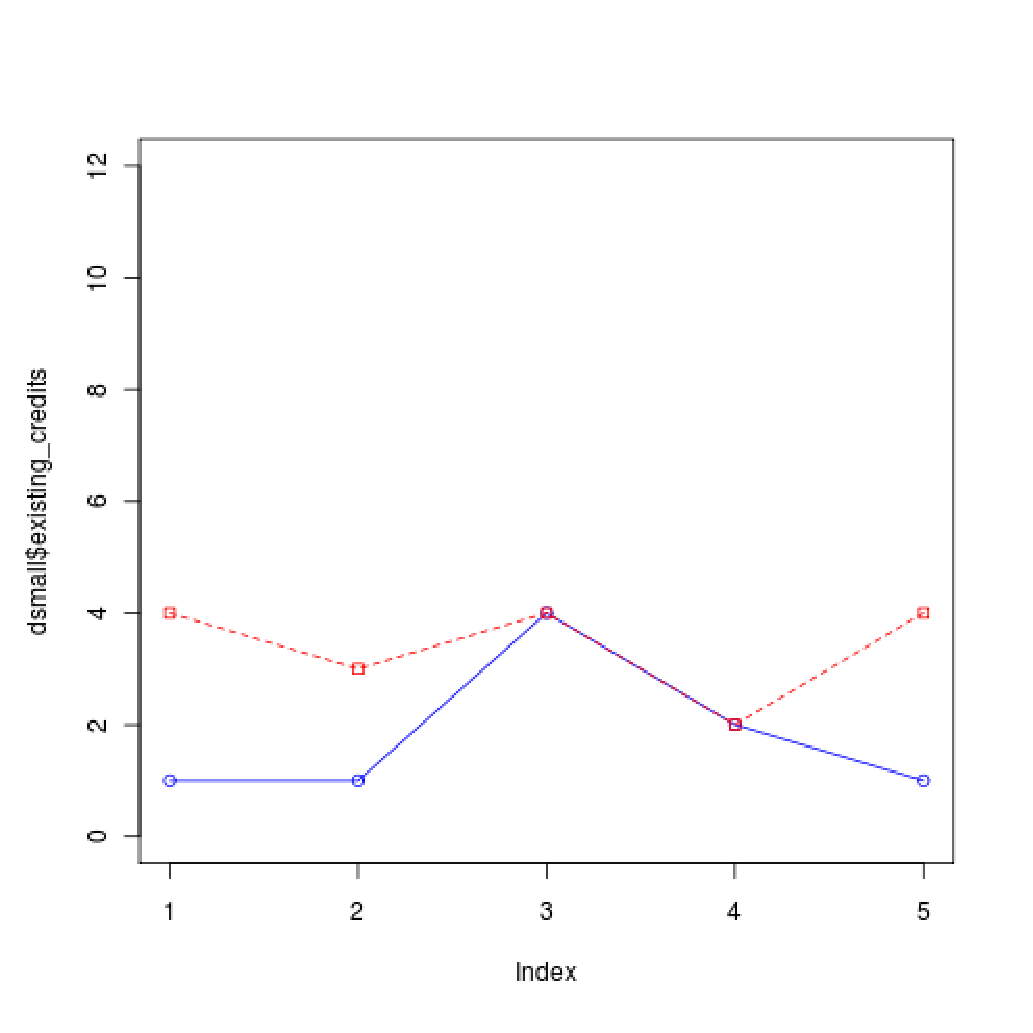
\includegraphics[keepaspectratio,width=4cm]{theimg/foo1c}}
 \caption{Puntos}
 \label{fig:puntos}
 \end{center}
\end{figure}

%-----
\subsection{Bigotes}

\begin{verbatim}
png(filename = "../figures/foo2.png")
boxplot(age)
\end{verbatim}

\begin{figure}[h]
 \centering
 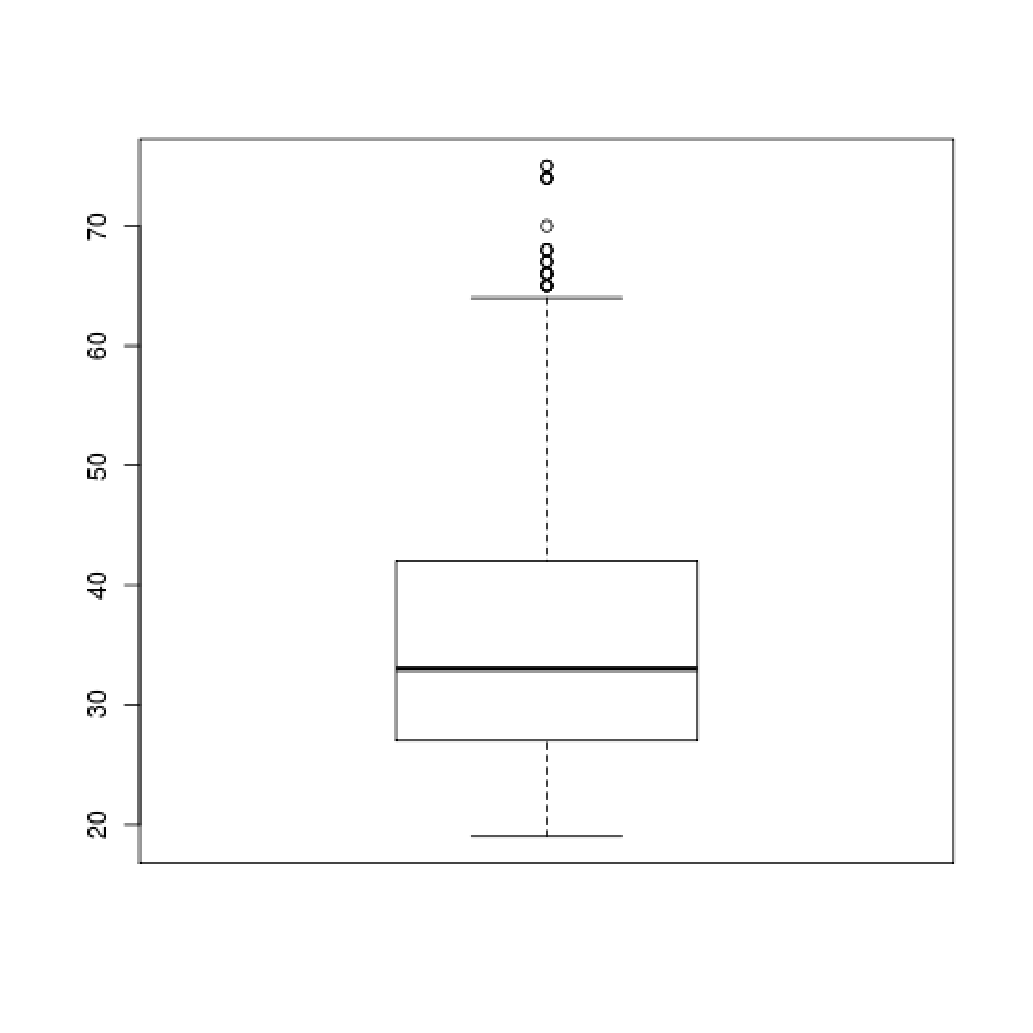
\includegraphics[keepaspectratio,width=5cm]{theimg/foo2}
 \caption[foo2]{foo2}
 \label{fig:bigos}
\end{figure}

%-----
\subsection{Histograma simple}

\begin{verbatim}
png(filename = "../figures/foo3.png")
hist(credit_amount)
\end{verbatim}

\begin{verbatim}
png(filename = "../figures/foo4.png")
hist(credit_amount, breaks=30, col="blue") 
\end{verbatim}

\begin{figure}[h]
 \begin{center}
 \subfigure[foo3]{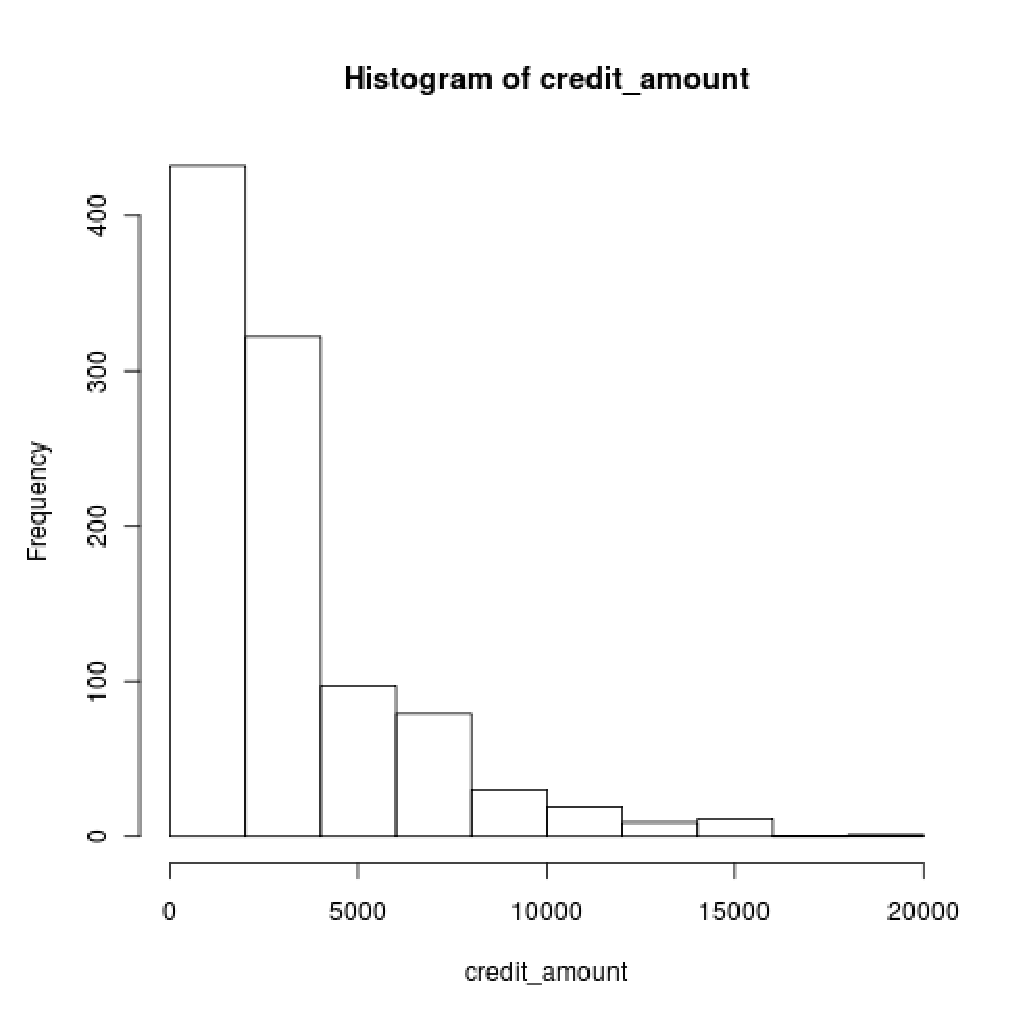
\includegraphics[keepaspectratio,width=6cm]{theimg/foo3}}
 \hspace{0.1cm}
 \subfigure[foo4]{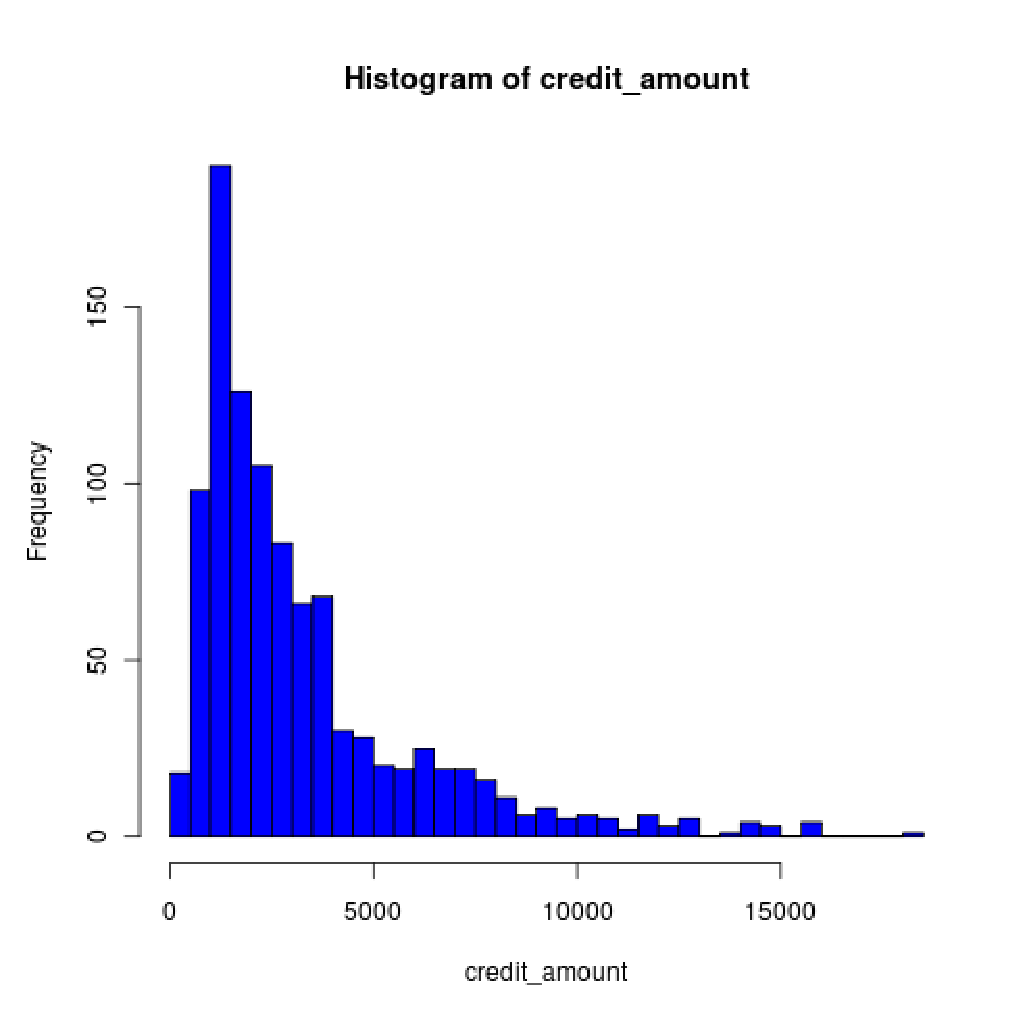
\includegraphics[keepaspectratio,width=6cm]{theimg/foo4}}
 \caption{Histograma}
 \label{fig:histograma}
 \end{center}
\end{figure}

%-----
\subsection{Barras}

\begin{verbatim}
png(filename = "../figures/foo5.png")
counts <- table(housing)
barplot(counts, main="Housing") 
\end{verbatim}

\begin{verbatim}
png(filename = "../figures/foo6.png")
counts <- table(class)
barplot(counts, main="Personal status", horiz=TRUE)
\end{verbatim}

\begin{verbatim}
png(filename = "../figures/foo6a.png")
myfile <- data.frame(dsmall$age,dsmall$residence_since,dsmall$duration)
barplot(as.matrix(myfile), main="Crédito", ylab= "Total",
   beside=TRUE, col=rainbow(5), cex.names=0.9)
legend("topright", c("e1","e2","e3","e4","e5"), bty="n", fill=rainbow(5))
\end{verbatim}

\begin{figure}[h]
 \begin{center}
 \subfigure[foo5]{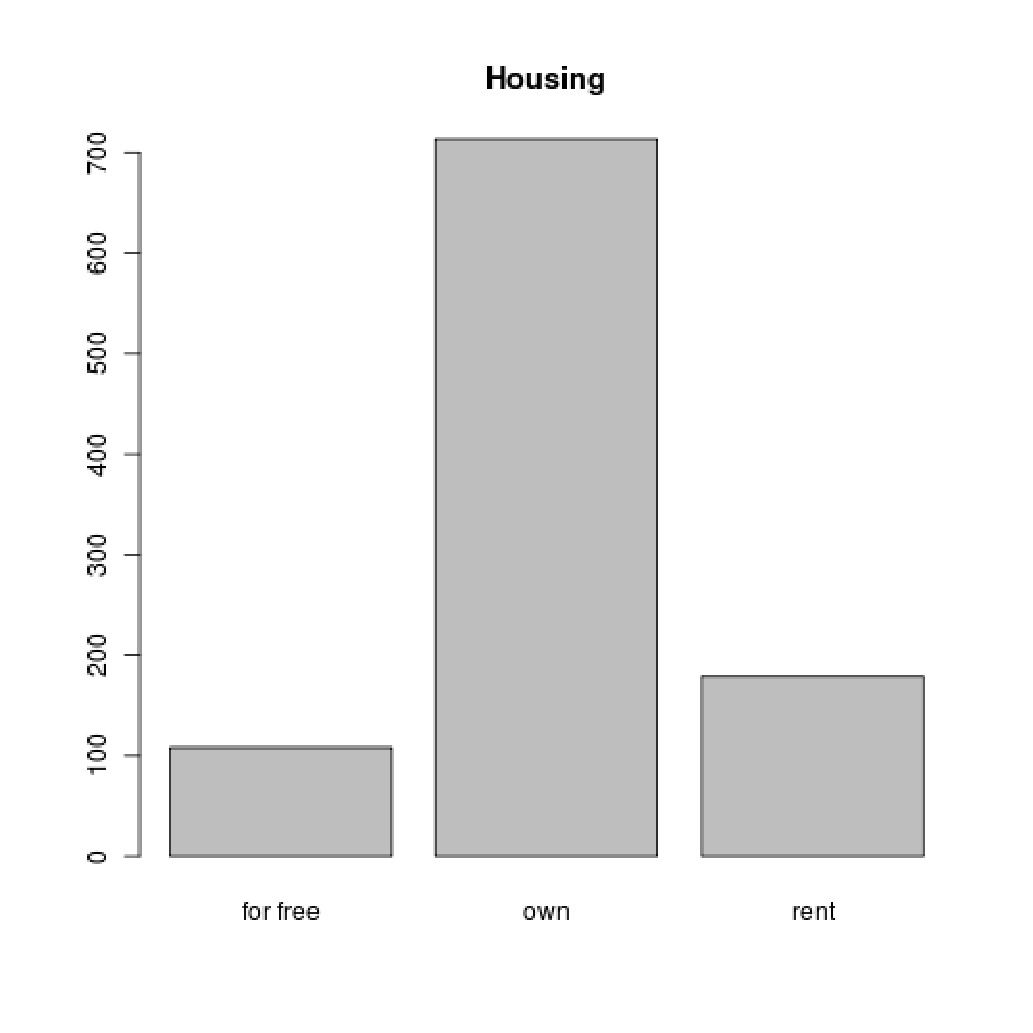
\includegraphics[keepaspectratio,width=4cm]{theimg/foo5}}
 \hspace{0.1cm}
 \subfigure[foo6]{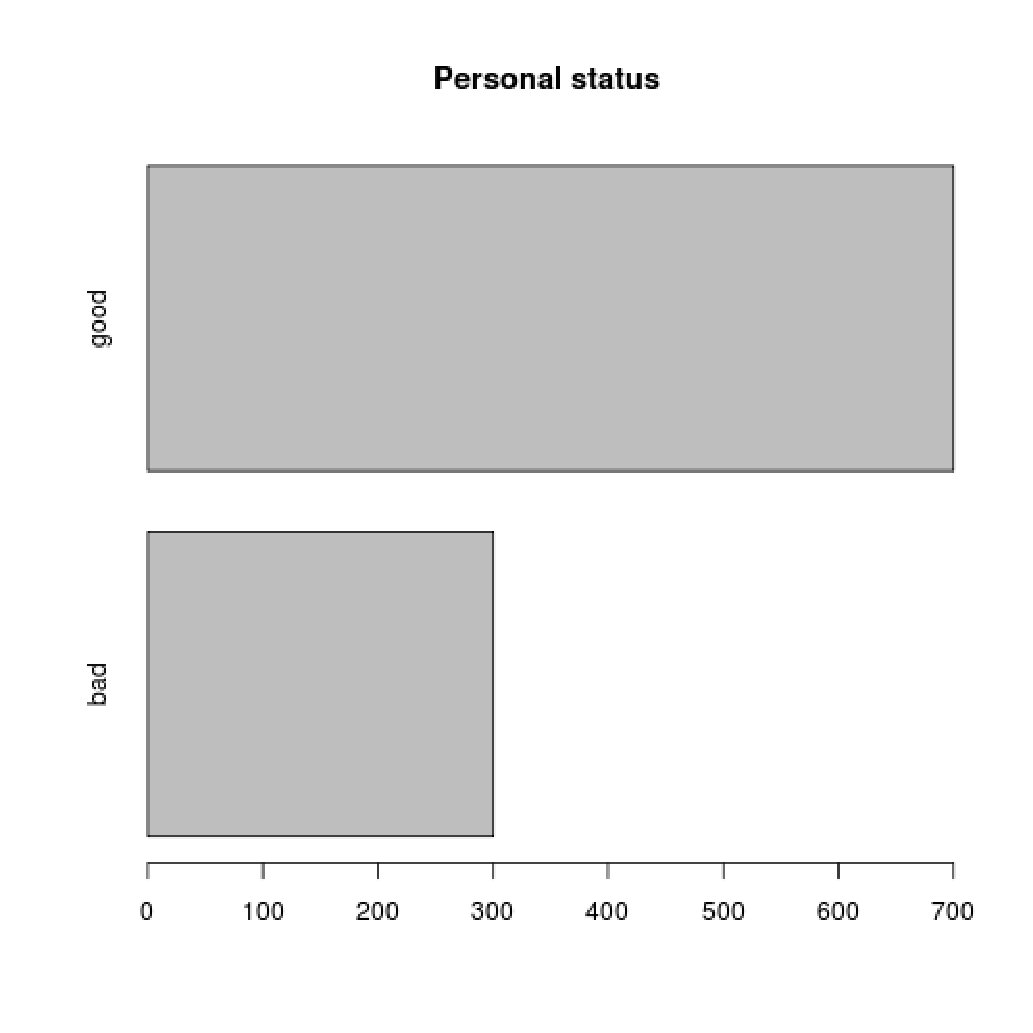
\includegraphics[keepaspectratio,width=4cm]{theimg/foo6}}
 \hspace{0.1cm}
 \subfigure[foo6a]{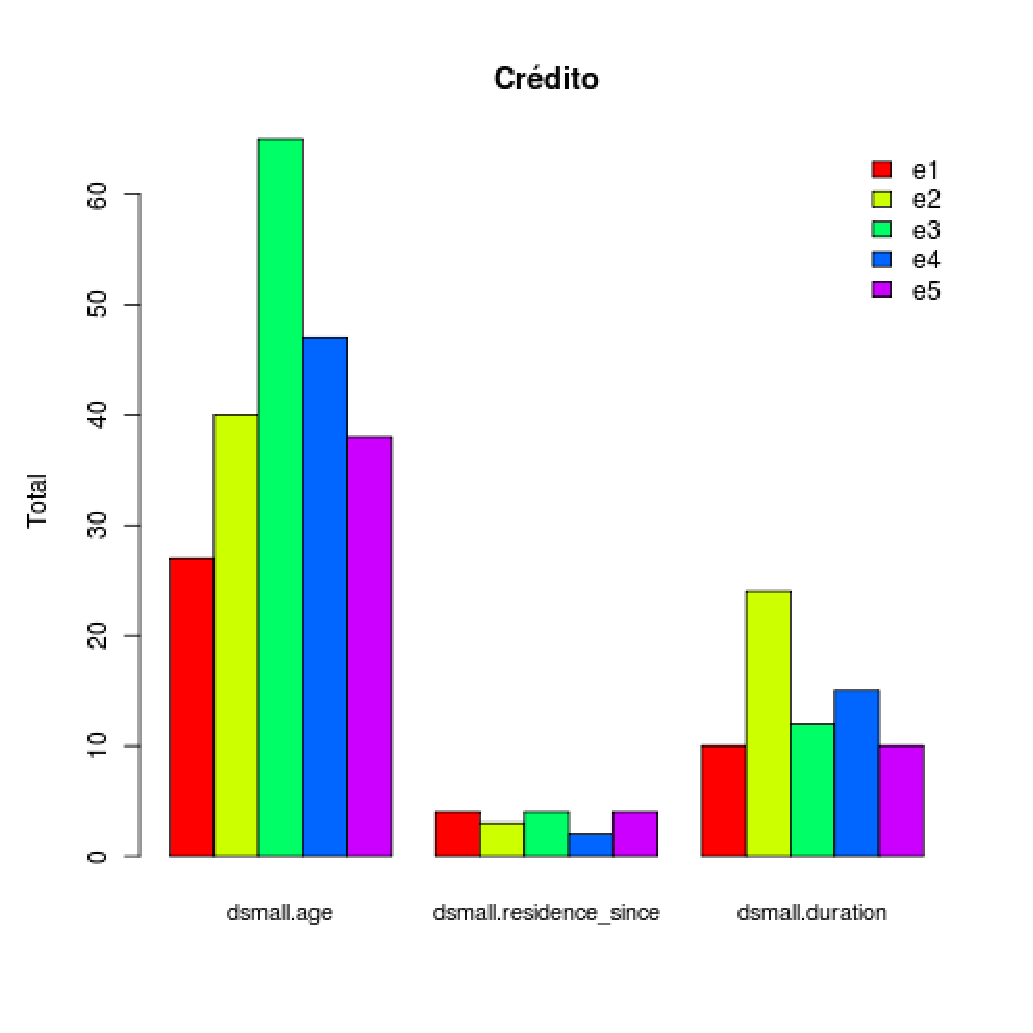
\includegraphics[keepaspectratio,width=4cm]{theimg/foo6a}}
 \caption{Barras}
 \label{fig:barras}
 \end{center}
\end{figure}

%-----
\subsection{Densidad}

\begin{verbatim}
png(filename = "../figures/foo7.png")
d <- density(credit_amount) # returns the density data
plot(d) # plots the results 
\end{verbatim}

\begin{verbatim}
png(filename = "../figures/foo8.png")
d <- density(credit_amount)
plot(d)
polygon(d, col="red") 
\end{verbatim}

\begin{figure}[h]
 \begin{center}
 \subfigure[foo7]{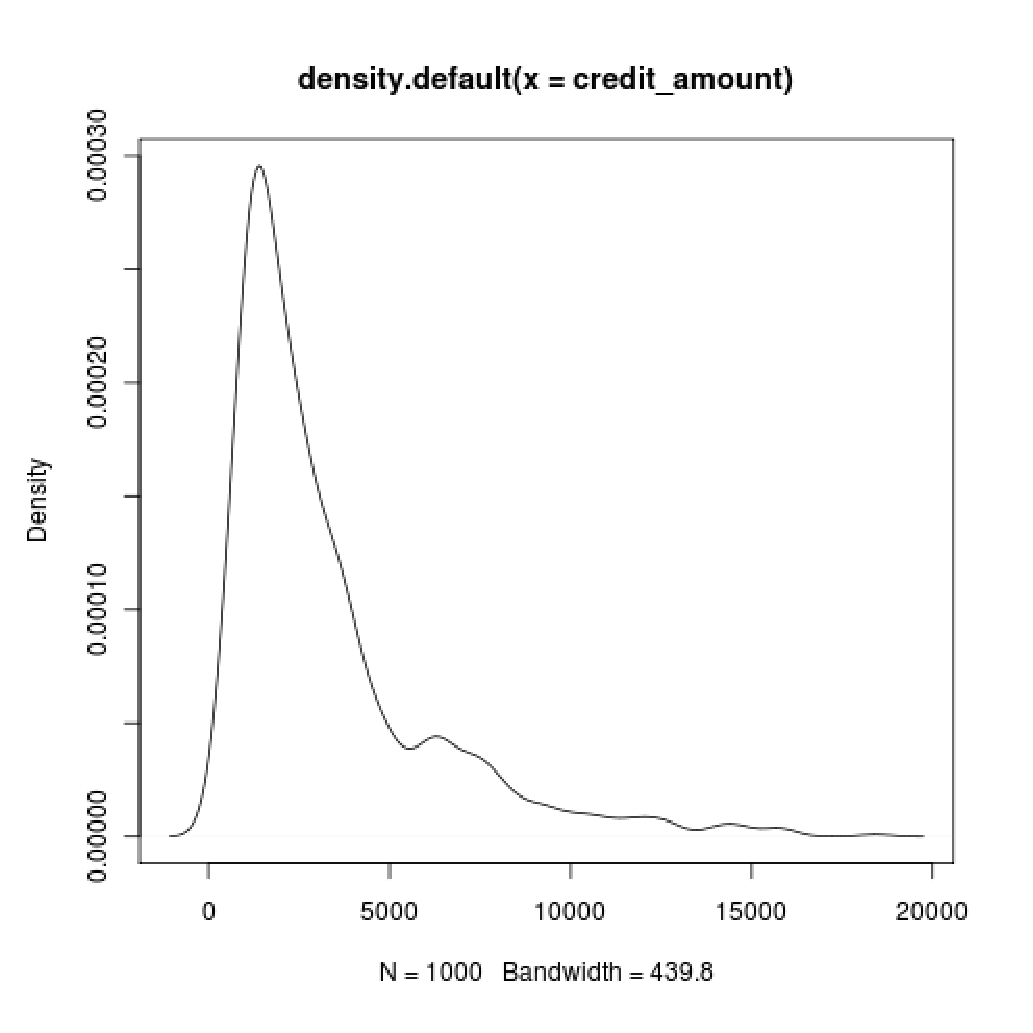
\includegraphics[keepaspectratio,width=5cm]{theimg/foo7}}
 \hspace{0.1cm}
 \subfigure[foo8]{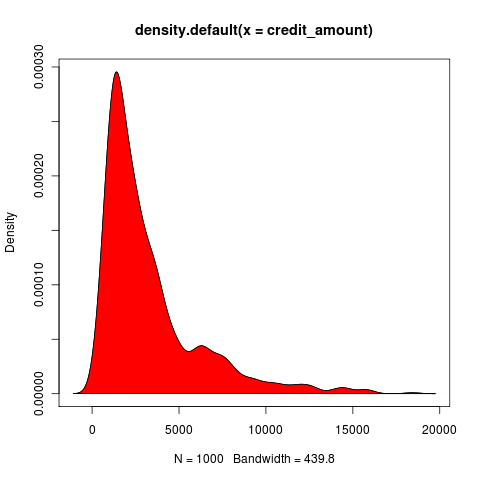
\includegraphics[keepaspectratio,width=5cm]{theimg/foo8}}
 \caption{Densidad}
 \label{fig:densidad}
 \end{center}
\end{figure}

%-----
\subsection{Matriz de dispersi'on}

\begin{verbatim}
png(filename = "../figures/foo9.png")
pairs(~credit_amount+age+existing_credits+num_dependents,data=credit,
   main="Simple Scatterplot Matrix")

\end{verbatim}

\begin{figure}[h]
 \centering
 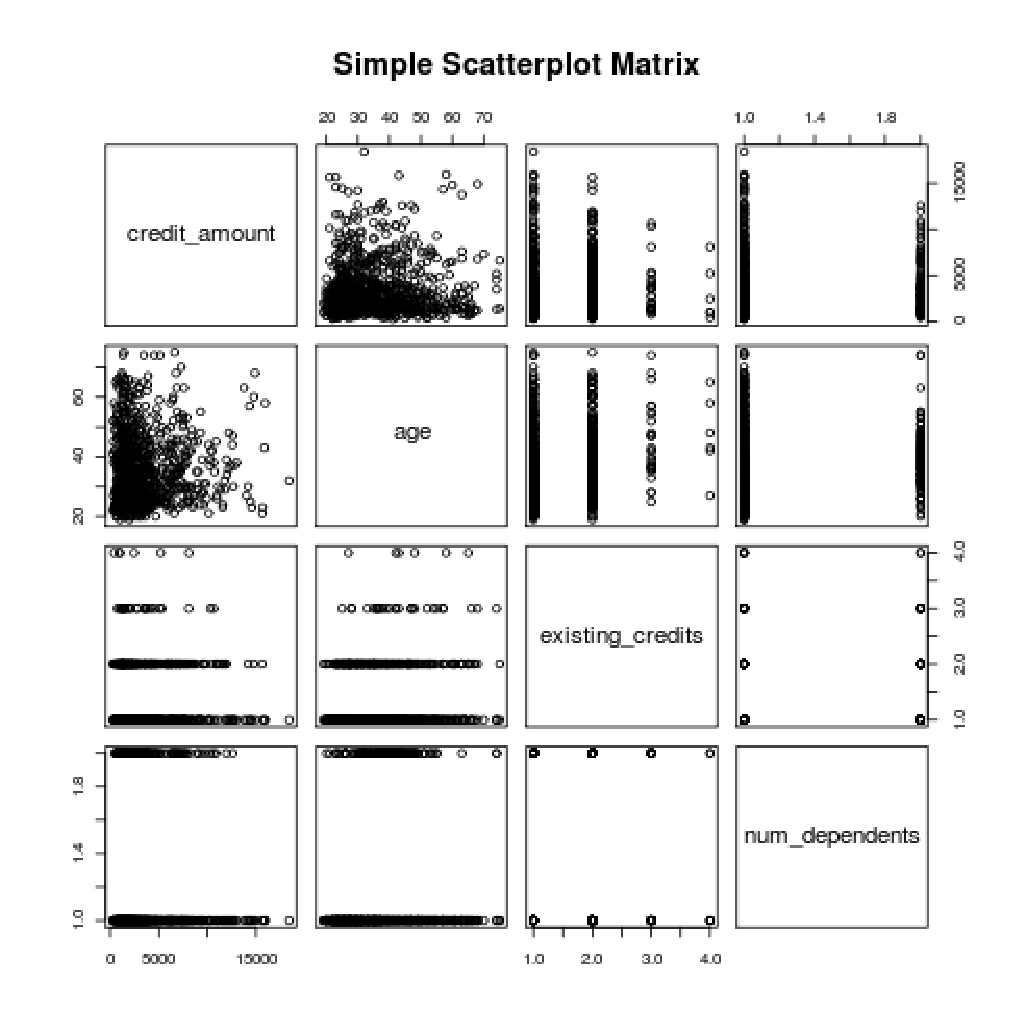
\includegraphics[keepaspectratio,width=7cm]{theimg/foo9}
 \caption[foo9]{foo9}
 \label{fig:puntos5}
\end{figure}


%-----------------------------------------------------------
\section{Librer'ia ggplot2}

%-----
\subsection{Bigotes}

\begin{verbatim}
d <- ggplot(data = credit, aes(x = credit_amount, y = age)) 
d + geom_boxplot(outlier.shape = 4) + theme_bw() + 
    scale_y_continuous(breaks = seq(0, 100, by = 5))
ggsave(file = "../figures/gg-boxplot.eps", width=5, height=5)
\end{verbatim}

%-----
\subsection{Barras}

\begin{verbatim}
d <- ggplot(data = credit, aes(age)) 
d + geom_bar() + theme_bw()
ggsave(file = "../figures/gg-foo10.eps", width=5, height=5)
\end{verbatim}

\begin{verbatim}
d <- ggplot(data = credit, aes(age)) 
d + geom_bar(binwidth = 0.1) + theme_bw()
ggsave(file = "../figures/gg-foo10a.eps", width=5, height=5)
\end{verbatim}

\begin{figure}[h]
 \begin{center}
 \subfigure[gg-boxplot]{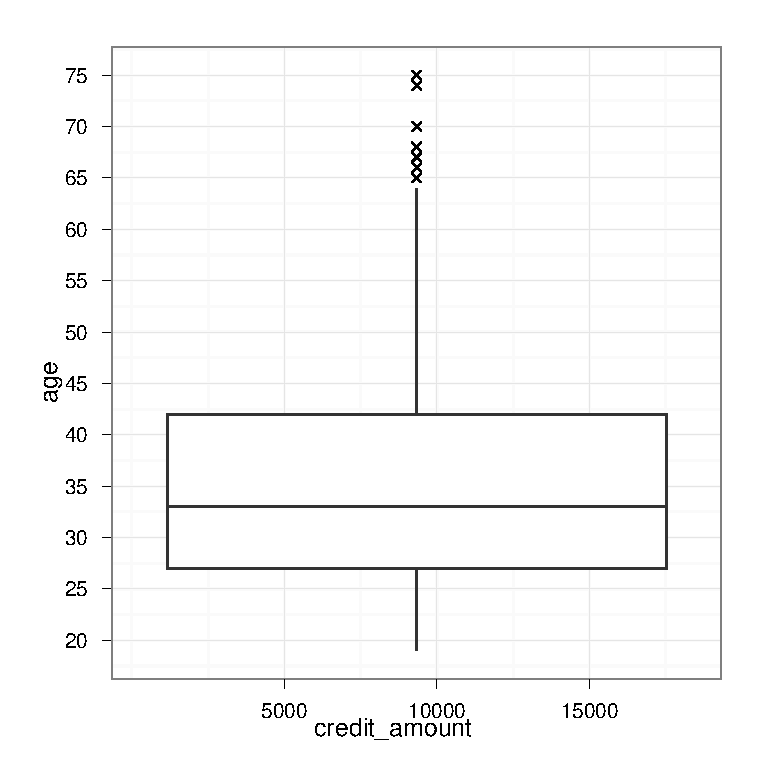
\includegraphics[keepaspectratio,width=4cm]{theimg/gg-boxplot}}
 \hspace{0.1cm}
 \subfigure[gg-foo10]{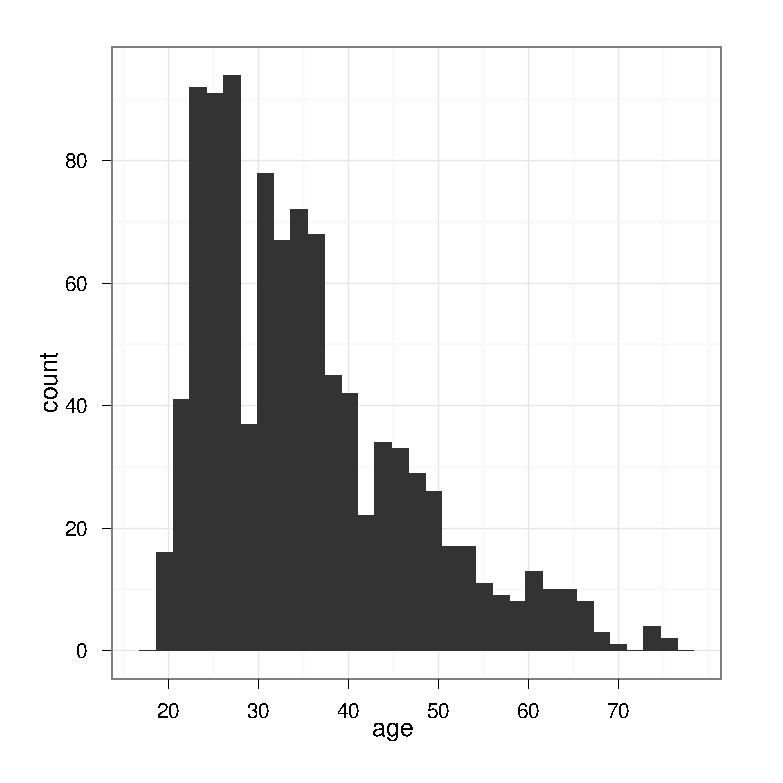
\includegraphics[keepaspectratio,width=4cm]{theimg/gg-foo10}}
 \hspace{0.1cm}
 \subfigure[gg-foo10a]{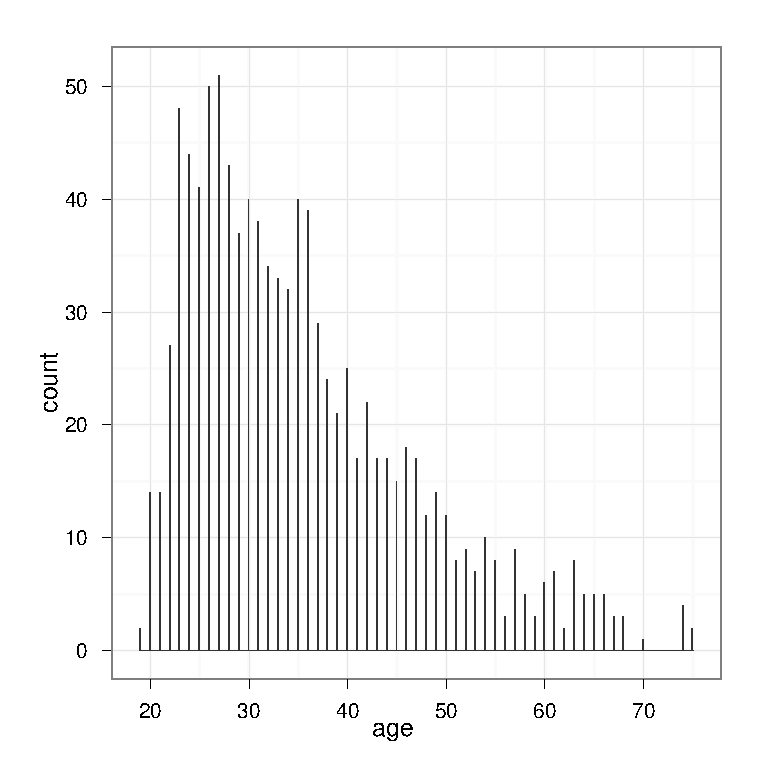
\includegraphics[keepaspectratio,width=4cm]{theimg/gg-foo10a}}
 \caption{Bigotes y barras}
 \label{fig:barras}
 \end{center}
\end{figure}

\begin{verbatim}
d <- ggplot(data = credit, aes(age)) 
d + geom_histogram(aes(y = ..count..),binwidth = 0.5)  + 
    theme_bw() + 
   scale_x_continuous(breaks = c(media)) + 
    geom_vline(xintercept = media, size = 0.5, colour = "magenta") +
    geom_vline(xintercept = media+sd, size = 0.5, colour = "blue", linetype = 2) +
    geom_vline(xintercept = media-sd, size = 0.5, colour = "blue", linetype = 2) 
ggsave(file = "../figures/gg-foo11.eps", width=5, height=5)
\end{verbatim}

\begin{figure}[h]
 \centering
 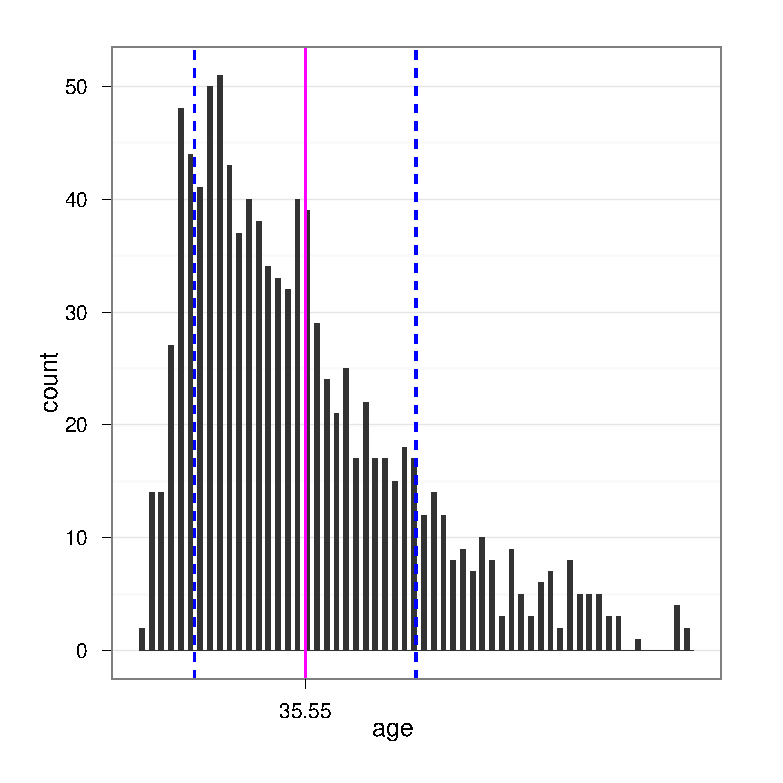
\includegraphics[keepaspectratio,width=6.5cm]{theimg/gg-foo11}
 \caption[foo11]{gg-foo11}
 \label{fig:foo11}
\end{figure}

\begin{verbatim}
agebin = cut(age,breaks = c(18,30,40,50,60,70,80))
agebinfile <- data.frame(purpose,credit_amount,personal_status,housing,job,
                         age=agebin,class)
agebinfile

d <- ggplot(data = agebinfile, aes(age)) 
d + stat_bin(aes(ymax = ..count..), geom = "bar") + theme_bw()
ggsave(file = "../figures/gg-foo12.eps", width=5, height=5)
\end{verbatim}

\begin{verbatim}
d <- ggplot(credit, aes(housing))
d + geom_bar()
ggsave(file = "../figures/gg-foo13.eps", width=5, height=5)
\end{verbatim}

\begin{figure}[h]
 \begin{center}
 \subfigure[gg-foo12]{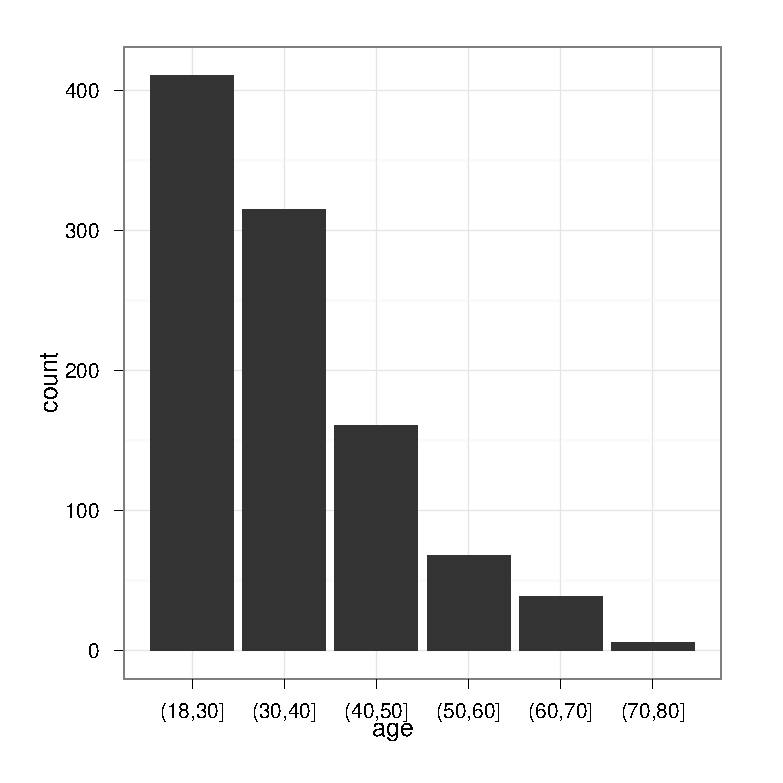
\includegraphics[keepaspectratio,width=5cm]{theimg/gg-foo12}}
 \hspace{0.1cm}
 \subfigure[gg-foo13]{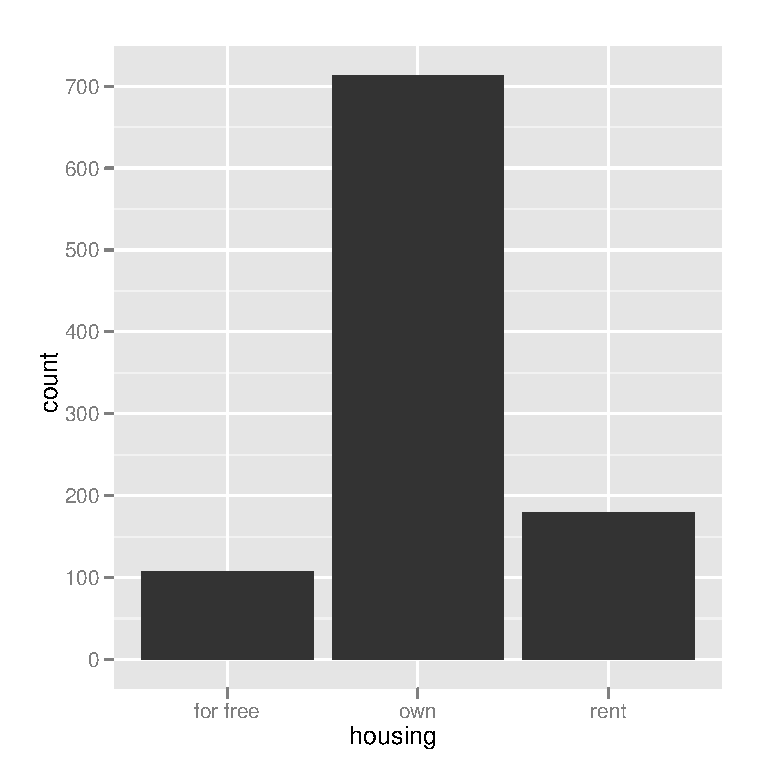
\includegraphics[keepaspectratio,width=5cm]{theimg/gg-foo13}}
 \caption{Barras}
 \label{fig:barras}
 \end{center}
\end{figure}

\begin{verbatim}
d <- ggplot(credit, aes(age,fill=housing))
d + geom_bar()
ggsave(file = "../figures/gg-foo14.eps", width=5, height=5)
\end{verbatim}

\begin{verbatim}
d <- ggplot(credit, aes(age))
d + geom_bar()+facet_wrap(~ housing)
ggsave(file = "../figures/gg-foo15.eps", width=5, height=5)
\end{verbatim}

\begin{figure}[h]
 \begin{center}
 \subfigure[gg-foo14]{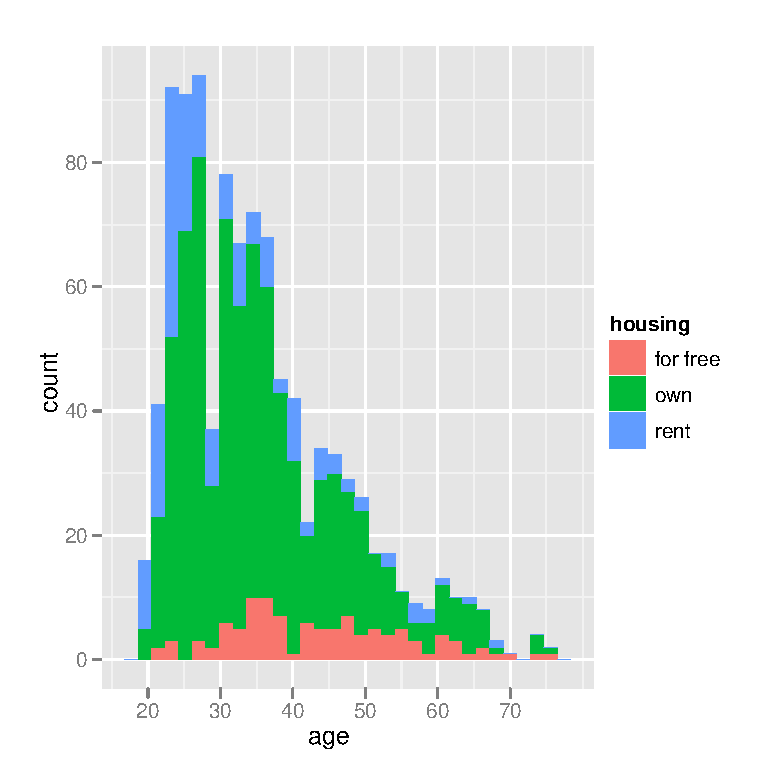
\includegraphics[keepaspectratio,width=7cm]{theimg/gg-foo14}}
 \hspace{0.1cm}
 \subfigure[gg-foo15]{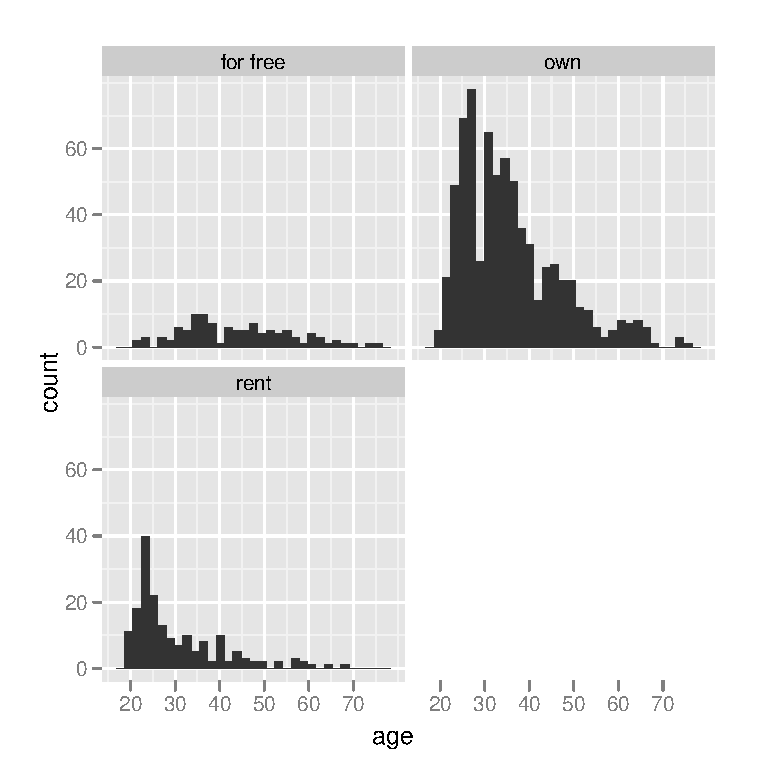
\includegraphics[keepaspectratio,width=7cm]{theimg/gg-foo15}}
 \caption{Barras y facetas}
 \label{fig:barras}
 \end{center}
\end{figure}




\chapter{Miner'ia de datos}

\url{http://www.the-data-mine.com/bin/view/Software/R}

%-----------------------------------------------------------
\section{Clasificaci'on}
Regresi'on lineal \url{http://www.youtube.com/watch?v=ZGTBOhbahmY}\\
\url{http://msenux.redwoods.edu/math/R/regression.php}\\
\url{http://scc.stat.ucla.edu/page_attachments/0000/0139/reg_1.pdf}\\

Arboles \url{http://en.wikibooks.org/wiki/Data_Mining_Algorithms_In_R/Classification/Decision_Trees}\\
\url{http://hisdu.sph.uq.edu.au/lsu/adrian/treecode.htm}\\
\url{http://www.statmethods.net/advstats/cart.html}\\

KNN \url{http://en.wikibooks.org/wiki/Data_Mining_Algorithms_In_R/Classification/kNN}


%-----
\section{Agrupaci'on}
KMeans \url{http://www.statmethods.net/advstats/cluster.html}\\
\url{http://stat.ethz.ch/R-manual/R-devel/library/stats/html/kmeans.html}\\
%-----
\section{Reglas de asociaci'on}

Apriori \url{http://prdeepakbabu.wordpress.com/2010/11/13/market-basket-analysisassociation-rule-mining-using-r-package-arules/}\\
\url{http://lyle.smu.edu/IDA/arules/}\\
\url{http://paginas.fe.up.pt/~ec/files_0506/R/arules.pdf}\\
\url{http://cran.r-project.org/web/packages/arulesViz/vignettes/arulesViz.pdf}\\
\url{http://www1.ccls.columbia.edu/~ansaf/lecture1.pdf}\\
%-----
\section{Selecci'on de atributos}

FSelector package \url{http://en.wikibooks.org/wiki/Data_Mining_Algorithms_In_R/Dimensionality_Reduction/Feature_Selection}\\

Caret package \url{http://cran.r-project.org/web/packages/caret/vignettes/caretSelection.pdf}\\

Boruta \url{http://www.jstatsoft.org/v36/i11/paper}\\
%-----
\section{Miner'ia de textos}
tm package \url{http://cran.r-project.org/web/packages/tm/vignettes/tm.pdf}\\

text mining infraestructure in R \url{http://www.jstatsoft.org/v25/i05/paper}\\

Rkea \url{http://cran.r-project.org/web/packages/RKEA/vignettes/kea.pdf}\\
%-----
\section{Otros tratamientos de los datos}
Machine Learning \url{http://cran.r-project.org/web/views/MachineLearning.html}\\

R with Python \url{http://www2.warwick.ac.uk/fac/sci/moac/students/peter_cock/r/rpy/}\\


Libro:\\
\url{http://www.r-bloggers.com/finally-a-practical-r-book-on-data-mining-data-mining-with-r-learning-with-case-studies-by-luis-torgo/}


http://www.johndcook.com/R_language_for_programmers.html\\

Data mining with R \url{http://cos.name/wp-content/uploads/2008/12/data-mining-with-r-by-john-maindonald.pdf}\\

Comparison: \url{http://brenocon.com/blog/2009/02/comparison-of-data-analysis-packages-r-matlab-scipy-excel-sas-spss-stata/}\\

Otros tratamientos: \url{http://www.statmethods.net/index.html}\\


%-----------------------------------------------------------
\addcontentsline{toc}{chapter}{\numberline{}Bibliograf'ia}
\bibliographystyle{apalike}
\bibliography{r}
%-----------------------------------------------------------
%\appendix
%\include{app1}

%-----------------------------------------------------------
\end{document}
%--------------------  Links
% http://www.statmethods.net/index.html
% http://www.gardenersown.co.uk/Education/Lectures/R/basics.htm
% http://www.harding.edu/fmccown/r/
% http://www.cyclismo.org/tutorial/R/index.html
%%% Funciones intro:
% http://cran.r-project.org/doc/manuals/R-intro.html#A-sample-session
%%% Posiblemente:
% http://www2.warwick.ac.uk/fac/sci/moac/degrees/modules/ch923/r_introduction/data_summary/
%%%%%%%%%%%%%%%%%%%%%%%%%%%%%%%%%%%%%%%%%%%%%%%%%%%%%%%%
% \begin{figure}[h]
% \centering
% \includegraphics[keepaspectratio,width=2cm]{theimg/bp}
% \caption[Bletchley Park]{Bletchley Park}
% \label{fig:bp}
% \end{figure}
%
% \begin{figure}[h]
% \begin{center}
% \subfigure[Teletipo]{\includegraphics[width=2.5cm,keepaspectratio]{theimg/teletipo}}
% \hspace{1cm}
% \subfigure[Colossus]{\includegraphics[keepaspectratio,height=2cm]{theimg/colossus}}
% \caption{Teletipo y Colossus}
% \label{fig:teletipocolossus}
% \end{center}
% \end{figure}
%
%\begin{table}[ht]
%\caption{Texto}
%\centering
%\begin{tabular}{c c c c}
%\hline\hline
%Case & Method\#1 & Method\#2 & Method\#3 \\ [0.5ex]
%\hline
%\end{tablular}
%\label{tab:example}
%\end{table}

